\documentclass[bachelor,german]{info1thesis}

%\usepackage[utf8]{inputenc}
%\usepackage[T1]{fontenc}
\usepackage{fontspec}
%\usepackage{lmodern} TODO: braucht man das?

\usepackage{tabularx}
\usepackage{ltablex}

\usepackage{path}
\usepackage{color}

\usepackage[disable,colorinlistoftodos]{luatodonotes}


%%%%%%%%%%%%%%%%%%%%%%%%%%%%%%%%%%%%%%%%%%%%%%%%%%%%%%%%%%%%%%%%%%%%%%%%%%%%%%%%
%%% Titelseite -- hier Titel und Autorennamen eintragen
\title{Leitfaden für Abschlussarbeiten} % Geben Sie hier den Titel Ihrer Arbeit an.
\subtitle{am Lehrstuhl für Informatik I}
\author{Benedikt Budig\and Fabian Lipp} % Geben Sie Ihren Namen an.
%\date{Eingereicht am \abgabedatum}
\titlehead{Julius-Maximilians-Universität Würzburg\\
Institut für Informatik\\
Lehrstuhl für Informatik I\\
Algorithmen, Komplexität und wissensbasierte Systeme}
\supervisors{Prof.\ Dr.\ Alexander Wolff\and
Max Mustermann, M.\,Sc.}

\begin{document}
%%%%%%%%%%%%%%%%%%%%%%%%%%%%%%%%%%%%%%%%%%%%%%%%%%%%%%%%%%%%%%%%%%%%%%%%%%
%%%%%%%%%%%%% Bitte nur ab hier Änderungen vornehmen %%%%%%%%%%%%%%%%%%%%%

\begin{abstract}
    Dieses Dokument soll Studenten an unserem Lehrstuhl bei der Erstellung
    ihrer Abschlussarbeit unterstützen.
    Wir zeigen eine beispielhafte Gliederung einer Arbeit und beschreiben
    die Inhalten der einzelnen Kapitel.
    Zusätzlich geben wir an vielen Stellen auch Hinweise zur Benutzung von
    \LaTeX\ für die Erstellung der Arbeit.
    Im Anhang~\ref{appendix:orga} geben wir ein paar Hinweise zum Ablauf der
    Betreuung von Abschlussarbeiten an unserem Lehrstuhl.

    \paragraph{Zur Handhabung dieses Pakets.}
    In diesem Paket sind Vorlagen für verschiedene Dokumenttypen enthalten, die
    sie als Ausgangspunkt für ihre Arbeit verwenden können.
    Es gibt jeweils Vorlagen für deutsche und englische Arbeiten.
    \begin{itemize}
        \item \verb+template_thesis_de.tex+, \verb+template_thesis_en.tex+:
            Vorlage für Bachelorarbeit bzw. Masterarbeit
        \item \verb+template_seminar_de.tex+, \verb+template_seminar_en.tex+:
            Vorlage für Seminarausarbeitungen und Praktikumsberichte
    \end{itemize}
    Der Quelltext zu diesem Leitfaden ist ebenfalls im Paket enthalten.
    Diesen können Sie als praktisches Beispiel dafür verwenden, wie diese
    Dokumentenklasse angewandt wird.

    \paragraph{Inhalt der Zusammenfassung.}
    Schreiben Sie hier eine Zusammenfassung der Arbeit, vergleichbar mit dem Abstract auf wissenschaftlichen Papers.
    Sie dient dem Leser dazu, einen groben Überblick über die Inhalte zu gewinnen (Problemstellung, verwendeter Lösungsansatz, ggf.\ experimentelle Ergebnisse, gewonnene Erkentnisse).
    Der Umfang soll ca.\ eine halbe Seite betragen.
    Für Seminararbeiten ist diese Zusammenfassung nicht erforderlich.
    
    \emph{Achtung:} Bei Arbeiten auf Englisch fordern die
    Prüfungsordnungen, dass es eine deutsche Zusammenfassung gibt.
    Schreiben Sie in diesem Fall eine englische \emph{und} eine deutsche Zusammenfassung (mit dem gleichen Inhalt).
    Die passenden \LaTeX-Befehle dafür finden Sie in den englischsprachigen
    Vorlagen.

    \paragraph{WARNUNG:} 
    Die vorliegende Version des Leitfadens ist eine \textcolor{red}{Vorabversion}, die noch nicht vollständig ist.
    Sie bezieht sich größtenteils auf die Ausarbeitung von Bachelor- und Masterarbeiten; Seminararbeiten unterscheiden sich davon etwas in Aufbau und Inhalt.

%    \vspace{3em}
%    \textbf{TODOs für die Titelseite:}
%    \todo{Soll der Name des Lehrstuhls für englische Arbeiten übersetzt werden?}
\end{abstract}

\thesistableofcontents






%%%%%%%%%%%%%%%%%%%%%%%%%%%%%%%%%%%%%%%%%%%%%%%%%%%%%%%%%%%%%%%%%%%%%%%%%%%%%%%%





%%%%%%%%%%%%%%%%%%%%%%%%%%%%%%%%%%%%%%%%%%%%%%%%%%%%%%%%%%%%%%%%%%%%%%%%%%%%%%%%
\chapter{Einleitung}
Das einleitende Kapitel der Arbeit beginnt mit einer Einführung in die Problemstellung bzw.\ einer Motivation für die vorliegende Forschung.
Dabei kann zum Beispiel auf die theoretische Relevanz oder auch in der Praxis relevante Anwendungen eines Problems verwiesen werden.
Es ist hilfreich, die Einleitung mit der Zusammenfassung der Arbeit und dem Schlusskapitel zu vergleichen. 
Damit stellt man sicher, dass diese inhaltlich im Bezug auf Zielsetzung und Motivation übereinstimmen. Dem Umfang sollte ca.\,5\% der gesamten Arbeit betragen.

\paragraph{Verwandte Arbeiten}
Anschließend werden verwandte Arbeiten, also Veröffentlichungen, die sich mit dem gleichen oder ähnlichen Themen beschäftigen, vorgestellt.
Dieser Abschnitt kann alternativ auch als eigenstehendes Kapitel nach der Einleitung in die Arbeit eingefügt werden, was besonders bei umfangreicheren Literaturrecherchen sinnvoll ist.
Nehmen Sie diesen Teil besonders ernst und recherchieren Sie gründlich.

Organisieren Sie die zitierte Literatur mit BibTeX und achten Sie darauf, die einzelnen Veröffentlichungen mit \emph{korrekten} und \emph{vollständigen} Angaben zu zitieren.
Tragen Sie bei einem Konferenzartikel neben Titel, Namen der Autoren und des Tagungsbandes gegebenenfalls auch die Namen der Herausgeber in die bib-Datei ein.
ISBN-Nummern sind nicht nötig.
Seien Sie vorsichtig mit Umlauten in der bib-Datei und besonders mit heruntergeladenen BibTeX-Referenzen von Verlagen und Suchmaschinen: diese sind sehr oft unvollständig und uneinheitlich.

Zitieren Sie stets so, dass der entsprechende Satz auch ohne die Rereferenzmarke noch Sinn ergibt; das Zitat soll eine Zusatzinformation sein. 
Also: "`Binucci et al.~\cite{bdln-odgvel-05} beschäftigen sich mit der Beschriftung von Graphen."'
Nicht: "`\cite{bdln-odgvel-05} beschäftigt sich mit der Beschriftung von Graphen."'
Wenn es von einem Artikel eine Konferenzversion \cite{bdln-lhod-02} und eine Zeitschriftenversion \cite{bdln-odgvel-05} gibt, so sollten Sie stets die Zeitschriftenversion (oder ein Buch \cite{gj-cigtn-79}) zitieren.

\todo[inline]{Wie Software zitieren? Paper dazu, Fußnote oder Literaturverzeichnis}
\todo[inline]{Beispiele für: Book, InProceedings, Article, Thesis}

\paragraph{Eigener Beitrag}
In der Einleitung ist es wichtig, den eigenen Beitrag zum eingeführten Problem klarzustellen.
Das funktioniert besonders gut, wenn die verwandten Arbeiten zuvor diskutiert wurden. 
Andernfalls sollte der eigene Beitrag trotzdem in der Einleitung erläutert und dann im Kapitel mit den verwandten Arbeiten mit diesen in Bezug gesetzt werden.

\paragraph{Aufbau der Arbeit}
Die Einleitung sollte mit einem kurzen Überblick über den Aufbau der Arbeit abgeschlossen werden.
Ein Beispielsatz: "`Zunächst werden grundlegende Definitionen eingeführt (Kapitel~\ref{chap:definitionen})."'


\chapter{Definitionen}
\label{chap:definitionen}
In fast allen Arbeiten wird mit grundlegenden Definitionen gearbeitet, welche dem Leser in diesem Kapitel nähergebracht werden sollen.
Vermeiden Sie eine lose Sammlung von Definitionen und Sätzen, sondern setzen Sie sie miteinander textuell in Bezug.
Zur Formatierung von Definitionen und Sätzen bieten sich die entsprechenden LaTeX-Umgebungen an:

\begin{definition}
  Dies ist ein Beispiel für eine Definition.
  Geben Sie auch für Definitionen möglichst eine Quelle an, z.\,B.\ ein entsprechendes Lehrbuch.
\end{definition}

Eine kurze Überleitung von einer Definition zu einem Satz hilft dem Leser zu verstehen, wohin die Reise gehen soll.
Beschränken Sie sich aber auf Definitionen und Sätze, die sie in späteren Teilen der Arbeit auch wirklich benötigen.

\begin{satz}[Beispielsatz] \label{thm:beispiel}
  Dies ist ein Beispiel für einen Satz.
\end{satz}

\begin{proof}
  Der Satz gilt offensichtlich, denn
  \begin{equation*}
    \sum_{i=1}^{n} 1 = n
  \end{equation*}
  Zudem wird der Beweis automatisch mit einem q.e.d.-Symbol beendet.
\end{proof}

Auf Sätze, wie z.\,B.\ Satz~\ref{thm:beispiel}, lässt sich mithilfe des Befehls \verb+\ref{labelname}+ verweisen, wenn man in der Satz-Umgebung einen "`Label"' mit \verb+\label{labelname}+ gesetzt hat. 
Genauso kann man auf Kapitel und Abschnitte, z.\,B. Kapitel~\ref{chap:definitionen}, verweisen.
%Üblicherweise beginnt man einen Labelnamen mit dem Typ der Umgebung, auf die man verweist, also z.\,B.\ \verb+\label{fig:trapez}+ für eine Abbildung (engl.\emph{figure}).
Zum Hervorheben (engl.\ \emph{emphasize}) eines \emph{neuen Begriffs} verwendet man den Befehl \verb+\emph{neuer Begriff}+, wenn der neue Begriff zum ersten Mal verwendet wird.


\chapter{Algorithmus}
Im Hauptteil Ihrer Arbeit werden Sie ein eigenes Forschungsergebnis präsentieren (oder, im Falle einer Seminarausarbeitung, das Hauptresultat Ihres Themas vorstellen).

\todo[inline]{Was muss hier noch alles hin?}

Vielleicht möchten Sie Ihren Algorithmus in Pseudocode angeben. 
Mit der \verb+algorithm+- Umgebung (aus dem Paket \verb+algorithm2e.sty+) ist es nicht schwer, Pseudocode in \LaTeX{} zu setzen (siehe Algorithmus~\ref{alg:binsearch}).

\begin{algorithm}
  \SetKw{True}{true}
  \SetKw{False}{false}
  \caption{BinäreSuche(Feld $A$, ganze Zahl $n$, Element $x$)}
  \label{alg:binsearch}
  \Ein{sortiertes Feld $A$, Länge $n$, gesuchtes Element $x$}
  \Aus{\True genau dann, wenn $x$ in $A$ enthalten ist}

  $l = 0$ \;
  $r = n-1$ \;

  \While{$l \le r$}{
    $m = \lfloor (l + r)/2 \rfloor$ \;
    \If{$A[m] == x$}{
      \Return \True \;
    }
    \ElseIf{$x < A[m]$}{
      $r = m - 1$ \;
    }
    \Else{
      $l = m + 1$ \;
    }
  }
  \Return \False
\end{algorithm}

\todo{Referenzen auf Zeilennummern erklären}
Das gleiche geht problemlos auch ohne Zeilennummern.  Dazu benützt man
einfach in der \verb+algorithm+-Umgebung den Befehl
\verb+\LinesNotNumbered+.


\chapter{Experimente}
Auch Abbildungen, wie z.\,B.\ Abbildung~\ref{fig:trapez}, sind schnell
eingefügt.  Wichtig: Fügen Sie eine Abbildung immer erst nach der
ersten Referenz auf die Abbildung ein!

\begin{figure}
  \centering
  \includegraphics[page=3]{abbildungen/trapez}
  \caption{Das ist eine Abbildung.}
  \label{fig:trapez}
\end{figure}

Im Allgemeinen braucht man die Endung der Bilddatei beim Einbinden mit
dem Paket \verb+\includegraphics+ nicht mit anzugeben.  Es empfiehlt
sich, alle Bilddateien in einen Unterordner abzulegen.  In mehrteiligen
Abbildungen kann man mit dem Paket \verb+subcaption+ jede mit einer
eigenen Bildunterschrift versehen.  Man kann sich dann im Text sowohl
auf die Teilabbildungen (z.\,B.\ Abbildung~\ref{fig:trapez-eins}) als
auch auf die Gesamtabbildung (z.\,B.\ Abbildung~\ref{fig:zwei-trapeze})
beziehen.

Wichtig: man sollte sich im Text auf jede Abbildung wenigstens einmal
beziehen.

\begin{figure}[h]
  \begin{subfigure}{.48\textwidth}
    \centering
    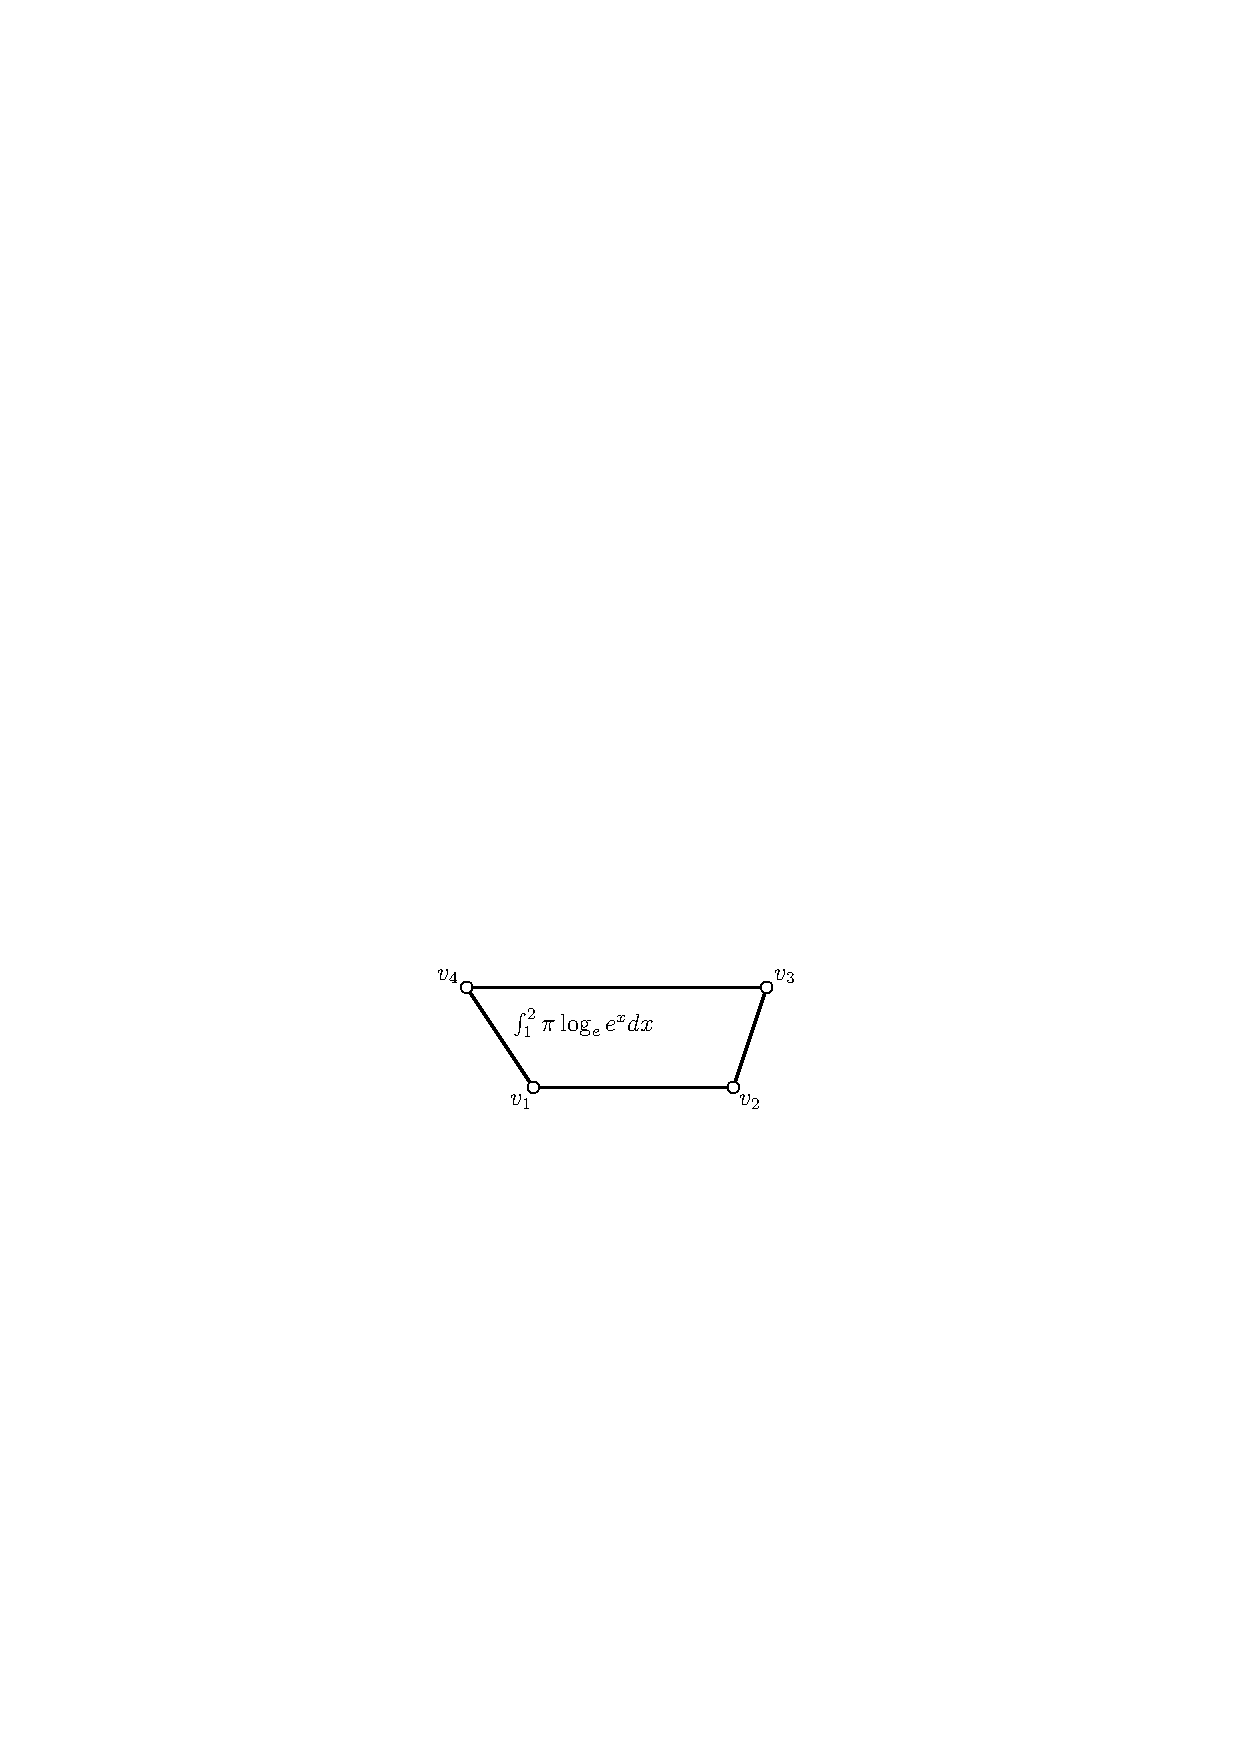
\includegraphics[page=1]{abbildungen/trapez}
    \caption{die erste Teilabbildung}
    \label{fig:trapez-eins}
  \end{subfigure}
  \hfill
  \begin{subfigure}{.48\textwidth}
    \centering
    \includegraphics[page=2]{abbildungen/trapez}
    \caption{die zweite Teilabbildung}
    \label{fig:trapez-zwei}
  \end{subfigure}
  \caption{Das ist eine Abbildung, die aus zwei Teilen besteht.}
  \label{fig:zwei-trapeze}
\end{figure}

\todo[inline]{Erkläre hier auch Tabellen. Erwähne: keine vertikalen Linien in Tabellen.}
\todo[inline]{Abbildungen und besonders Tabellen müssen im Text erklärt/interpretiert werden.}

\chapter{Zusammenfassung und Ausblick}
Schließen Sie Ihre Arbeit mit einer Zusammenfassung und einem Ausblick auf zukünftige Forschung ab.
In der Zusammenfassung sollen die Problemstellung, Ihr gewählter bzw.\ entwickelter Ansatz und die Ergebnisse deutlich werden.
Es ist hilfreich, die Einleitung mit der Zusammenfassung der Arbeit und dem Schlusskapitel zu vergleichen. 
Damit stellt man sicher, dass diese inhaltlich im Bezug auf Zielsetzung und Motivation übereinstimmen. Dem Umfang sollte ca.\,5\% der gesamten Arbeit betragen.

\paragraph{Ausblick} Schreiben Sie für den Ausblick (auf Englisch: \emph{future work}) einen eigenen Absatz. 
Sie können hier eine Einschätzung der Limitationen Ihrer Forschung abgeben und Ideen zu zukünftigen Weiterentwicklungen oder Anwendungen Ihrer Ergebnisse präsentieren.
Auch offene Fragen können hier stehen, wodurch Sie Ihre Ergebnisse noch einmal klar von ähnlichen Problemstellungen abgrenzen.


%%%%%%%%%%%%%%%%%%%%%%%%%%%%%%%%%%%%%%%%%%%%%%%%%%%%%%%%%%%%%%%%%%%%%%%%%%%%%%%%
\thesisbibliography
\bibliography{leitfaden}



\appendix


\chapter{Formelles/LaTeX}
In diesem Anhang haben wir noch einige Formalitäten beschrieben, die Sie beim
Schreiben Ihres Textes beachten sollten.
Außerdem listen wir noch Beispiele für häufig gemachte Fehler bei der
Verwendung von \LaTeX{} auf.

\paragraph{Gliederung.} Fangen Sie ein Kapitel nicht gleich mit einem
Abschnitt an, sondern sagen Sie zuerst etwas über den Inhalt des ganzen
Kapitels.
Ein Beispiel: "`Wir werden uns im Folgenden mit der Erweiterung des XY-Algorithmus auf unsere Problemstellung beschäftigen."'

Vermeiden Sie zu viele Unterebenen; das macht Ihre Arbeit nicht unbedingt
übersichtlicher.
In kurzen Arbeiten (z.\,B.\ Seminarausarbeitungen) sollten Sie nicht mehr als
zwei Gliederungsebenen verwenden.
In längeren Arbeiten können in manchen Fällen auch drei Ebenen sinnvoll sein.
Verwenden sie also keinesfalls Ebenen tiefer als \verb+\subsection+.
Die Verwendung von \verb+\paragraph+ kann helfen, Text in kleinere Einheiten zu gliedern, ohne eine eigene Gliederungsebene verwenden zu müssen.

\paragraph{Schreibkonventionen.} Gerade bei mathematischen Texten mit ihrer
speziellen Notation gibt es einige Konventionen, die dem Leser das
Verständnis erleichtern.  Darum geht es in der folgenden
Tabelle\footnote{Autor: Alexander Wolff}:
\todo{Seitenumbruch in Tabelle}

\bgroup
\setlength{\parskip}{1ex}
\setlength{\parindent}{0ex}
\setlength{\extrarowheight}{1ex}
\newcounter{myctr}
\setcounter{myctr}{0}
\newcommand{\regel}[1]{\multicolumn{3}{@{}l}{\addtocounter{myctr}{1}\arabic{myctr}.) #1}\\}
\begin{tabularx}{\textwidth}{@{}p{1ex}XX@{}}
  \em \# & \em schlechtes Beispiel & \em gutes Beispiel
  \\[1ex]\hline\\[-2ex]

  \regel{Spellchecker benutzen!!!}

  %& \multicolumn{2}{l}{In Unix z.B.\ so:
  %  \path+cat datei.tex | ispell -t -l -C -d german -T latin1 | sort -u+} \\

  \regel{Keine Variablen am Satzanfang!}

  & bla bla. $\theta$ ist hier wichtig.
  & bla bla. Der Parameter $\theta$ ist hier wichtig. \\

  \regel{Worte, die betont werden sollen, mit \verb+\emph+ kursiv
  setzen, nicht fett!}

  & Für \textbf{gerade} Werte... & Für \emph{gerade} Werte... \\

  \regel{Worte, die neu eingeführt oder definiert werden, mit
  \verb+\emph+ setzen!  (Aber nur einmal!)}

  & Ein Graph ist ein Tupel $(V,E)$...
  & Ein \emph{Graph} ist ein Tupel $(V,E)$... \\

  \regel{Dies gilt auch in einer \verb+definition+-Umgebung!}

  & \emph{Ein Graph ist ein Tupel $(V,E)$...}
  & \emph{Ein \emph{Graph} ist ein Tupel $(V,E)$...} \\

  \regel{Keine Quantoren, Folgerungspfeile und Vergleichsoperatoren im
    Fließtext verwenden!}

  & Dies gilt $\forall x \in \mathbb{R}$.
  & Dies gilt für alle $x \in \mathbb{R}$. \\[-1ex]
  & $a > b - c \Leftrightarrow a+c > b$
  & $a > b - c$ ist äquivalent zu $a+c > b$. \\[-1ex]
  & Der Faktor ist $>3$.
  & Der Faktor ist größer als $3$.  Es gilt $f>3$. \\

  \regel{Brüche im Fließtext nicht mit \verb+\frac+ setzen!}

  & Für $\tau \ge \frac{1}{\pi^2}$ gilt...
  & Für $\tau \ge 1/\pi^2$ gilt... \\

  \regel{Wörter oder Abkürzungen im Mathe-Modus (\verb+$...$+)
    mit \verb+\mathrm+ setzen!}

  & $\sigma_{opt} = |CH(P)|$
  & $\sigma_\mathrm{opt} = |\mathrm{CH}(P)|$\\

  \regel{In mathematischen Aufzählungen \verb+\dots+ statt "`..."'
    verwenden!}

  & $p_1, ..., p_n$ und $x_1 + ... + x_m$
  & $p_1, \dots, p_n$ und $x_1 + \dots + x_m$ \\

  \regel{Satzzeichen (nicht aber Klammern) ohne Lücke an das
  vorstehende Wort anschließen!}

  & Das ist doch(sicher) klar , oder ? & Das ist doch (sicher) klar, oder? \\

  \regel{Anzahlen (nicht aber Zahlen) bis zwölf ausschreiben!}

  & Die 3 Knoten haben Grad 3.
  & Die drei Knoten haben Grad 3. \\

  \regel{In Mengendefinitionen \verb+\mid+ statt $|$ verwenden!}

  & $A_y = \{ x \in B | x \le y \}$
  & $A_y = \{ x \in B \mid x \le y \}$ \\

  \regel{In \LaTeX\ vordefinierte Funktionsnamen wie \verb+\max+,
    \verb+\log+ oder \verb+\det+ verwenden!}

  & $sup_{x>0} max \{ cos x, sin x \} = 1$
  & $\sup_{x>0} \max \{ \cos x, \sin x \} = 1$ \\

  \regel{Doppelindizes wenn möglich vermeiden!}

  & $a_{i_j}$
  & $a_{i,j}$ oder $a_{\sigma(i)}$ für $\sigma \in S_n$ \\

  \regel{Für Zahlensysteme \verb+\mathbb+ aus dem Paket \verb+amssymb+
    verwenden!}

  & $N, Z, Q, R, C$
  & $\mathbb{N}, \mathbb{Z}, \mathbb{Q}, \mathbb{R}, \mathbb{C}$ \\

  \regel{Wörter, die \emph{ein} Ding bezeichnen, zusammenschreiben
    oder Bindestriche verwenden!}

  & Der Fair Split Tree ist eine Daten Struktur.
  & Der Fair-Split-Tree ist eine Datenstruktur. \\

  \regel{Unterschied zwischen verschiedenen Stricharten machen!}

  & Seiten 5-6 sind - denke ich - wichtig.
  & Seiten 5--6 sind~-- denke ich~-- wichtig. \\[-1ex]
  & Taschen und Deckenlampen erleuchten.
  & Taschen- und Deckenlampen erleuchten.\\

  \regel{Höchstens sehr gebräuchliche Abkürzungen (bzw., usw.) verwenden!}

  & $\Rightarrow$ OBdA. & Daraus folgt ohne Beschränkung der ... \\

  \regel{Abstand zwischen Satzpunkt (\verb+.+) und Abkürzungspunkt
    (\verb+.\ +) unterscheiden!}

  & A, B, usw. \hspace{.1ex} lernen gerne \LaTeX.  \hspace{.1ex} Aber Z...
  & A, B, usw.\ lernen gerne \LaTeX.  \hspace{.1ex} Aber Z...\\

  \regel{Je nach Sprache korrekte Anführungszeichen verwenden!}
  
  & (\verb+''engl.''+~-- \verb+"`dt."'+~-- \verb+"<fr.">+) \\
  
  & ''Sure!''~-- ``Aber ja!''~-- ''Mais oui!''
  & ''Sure!''~-- "`Aber ja!"'~-- "<Mais oui!"> \\

  \regel{Für Tabellen, bei denen eine Spalte den "`Rest"' des Platzes verwenden soll:}
  
  & Paket \verb+tabularx+! \\

  \regel{Absätze nicht durch \verb+\\+ sondern durch eine Leerzeile beenden!}
  
  & (\texttt{\verb+\ +setlength\{\verb+\ +parskip\}\{1ex\}}) \\

  \regel{Absätze, die nur aus ein, zwei Zeilen bestehen, wenn möglich
    vermeiden!}

  \regel{Abbildungen mit einer aussagekräftigen Bildunterschrift
    (\verb+\caption+) versehen.}

  \regel{Im Fließtext auf \emph{jede} Abbildung Bezug nehmen:
    \verb+siehe Abbildung~\ref+\verb+{fig:super}+}

\end{tabularx}
\egroup


\chapter{Organisatorisches}
\label{appendix:orga}

In diesem Abschnitt beschreiben wir, wie wir uns die Betreuung vorstellen, um
Sie bestmöglich unterstützen zu können.

\section{Formalia}
Die Abschlussarbeit muss zum Beginn im Prüfungsamt angemeldet werden.
Dabei wird das Thema festgelegt und mit der Anmeldung beginnt auch die
Bearbeitungsdauer und die Abgabefrist wird festgelegt.
Wir geben Ihnen vor der Anmeldung einige Wochen Zeit, um mit dem Thema vertraut
zu werden und Literatur zu sichten.
Erst dann müssen Sie sich festlegen, ob Sie die Abschlussarbeit tatsächlich bei
uns schreiben möchten.
Nach Ihrer Entscheidung erfolgt die Anmeldung zeitnah, damit die Arbeiten 
vergleichbar bleiben und Sie Sicherheit für Ihre persönliche Zeitplanung 
haben. 

Beachten Sie bei der Abgabe der Arbeit die Regularien, die in der für Sie
gültigen Prüfungsordnung (fachspezifische Bestimmungen und ASPO) festgelegt
sind.


\section{Git-Repository}
Zur Verwaltung der Dateien für Ihre Abschlussarbeit sollten Sie ein
Git-Repository verwenden.
Dieses können Sie auf dem GitLab-Server des Instituts für Informatik anlegen.
Fügen Sie ihre Betreuer als Mitglieder zum GitLab-Projekt hinzu, damit wir Ihre
Fortschritte verfolgen können und ggf.\ bei technischen Problemen einfacher
helfen können.
Weitere Hinweise zur Verwendung von Git:
\begin{itemize}
    \item Verwenden Sie aussagekräftige Commit-Beschreibungen.

    \item Legen Sie keine automatisch erzeugten Dateien im Repository ab.
        Das betrifft beispielsweise von LaTeX erzeugte Dateien (\texttt{*.toc},
        \texttt{*.log}, \texttt{*.aux}, \dots).
        Auch die erzeugte PDF Ihrer Abschlussarbeit (für die ja der Quelltext
        im Repository liegt) sollten Sie nicht ins Repository einchecken.

        Falls Sie im Rahmen ihrer Abschlussarbeit etwas programmieren, legen
        Sie nur Quelltexte im Repository ab, keine kompilierten Programme.

    \item Sie können eine \texttt{.gitignore}-Datei anlegen, um bestimmte
        Dateien/Pfade/Muster dauerhaft aus dem Repository auszuschließen.
\end{itemize}
Stellen Sie die Änderungen an Ihrem Text regelmäßig ins Repository, damit wir
mitlesen können.
Wir versuchen ab und zu auf Ihre bisherige Arbeit zu schauen und Ihnen
Rückmeldungen dazu zu geben, um den Text zu verbessern.


\section{Regelmäßige Treffen}
In der Regel treffen Sie sich wöchentlich mit Ihren Betreuern um den aktuellen
Stand, mögliche Probleme, Lösungsansätze und Ideen für die weitere Arbeit zu
besprechen.
Normalerweise versuchen wir einen festen Termin für jede Woche zu vereinbaren.
Diese Treffen sollten Sie in einem kurzen Protokoll schriftlich festhalten,
damit wir auch nach ein paar Wochen noch nachvollziehen können, was besprochen
wurde.
Dazu bietet sich beispielsweise ein LaTeX-Dokument im Git-Repository an, dem
Sie nach jedem Treffen einen Abschnitt hinzufügen.
Dafür können Sie sich an folgendem Aufbau orientieren (die ersten Punkte
können Sie sinnvollerweise schon vor dem Treffen eintragen):
\begin{itemize}
    \item Fortschritte: Was haben Sie in der vergangenen Woche erreicht? Welche
        neuen Resultate wollen Sie uns zeigen?
    \item Probleme: Gibt es irgendwelche Probleme, bei denen Sie nicht
        weiterkommen?
    \item Inhalte des Treffens: Was haben wir diskutiert? Welche neuen Ideen
        sind entstanden?
    \item Ziele für nächste Woche: Woran wollen Sie bis zum nächsten Treffen
        arbeiten?
    \item Weitere Ideen: Welche weiteren Ideen (die nicht in den nächsten Wochen
        umgesetzt werden können) kamen noch auf?
\end{itemize}

Wenn Sie Änderungen wenigstens 24 Stunden vor dem Treffen ins Repository
pushen, versuchen wir vor dem Treffen noch darauf zu schauen.


\section{Mittagsseminar}
Bei uns am Lehrstuhl findet gelegentlich das Mittagsseminar statt.
In diesem Rahmen halten Mitarbeiter und Gäste Vorträge zu Ihrer aktuellen
Forschung.
Die Vorträge finden üblicherweise vor dem Mittagessen statt und werden über
einen Mailverteiler angekündigt, zu dem wir Sie mit Beginn Ihrer Arbeit
hinzufügen.
Wir freuen uns immer, wenn interessierte Studenten an den Vorträgen teilnehmen.

Außerdem laden wir Sie auch herzlich ein, im Rahmen Ihrer Abschlussarbeit selbst
einen kurzen Vortrag in diesem Rahmen zu halten.
Auf diese Weise können Sie Ihre Vortragsfähigkeiten trainieren und in
der anschließenden Diskussion auch hilfreiche Anregungen für Ihre
Abschlussarbeit erhalten.
Sprechen Sie uns bei Interesse einfach an!


\section{Veröffentlichung der Arbeit auf unserer Homepage}
Wir würden uns freuen, wenn wir auch Ihre Abschlussarbeit auf unserer
Lehrstuhl-Homepage\footnote{\url{http://www1.informatik.uni-wuerzburg.de/abschlussarbeiten/}}
veröffentlichen können.
Dazu bitten wir Sie nach Abschluss Ihrer Arbeit ein Formular auszufüllen, das
uns diese Veröffentlichung gestattet.

%\clearpage
%\pdfbookmark[0]{ToDo-Liste}{todos}
%\listoftodos

\end{document}
